\documentclass[tikz,border=6pt]{standalone}
\usepackage{amsmath}
\usepackage{xcolor}

\definecolor{blockblue}{HTML}{4A90D9}

\begin{document}
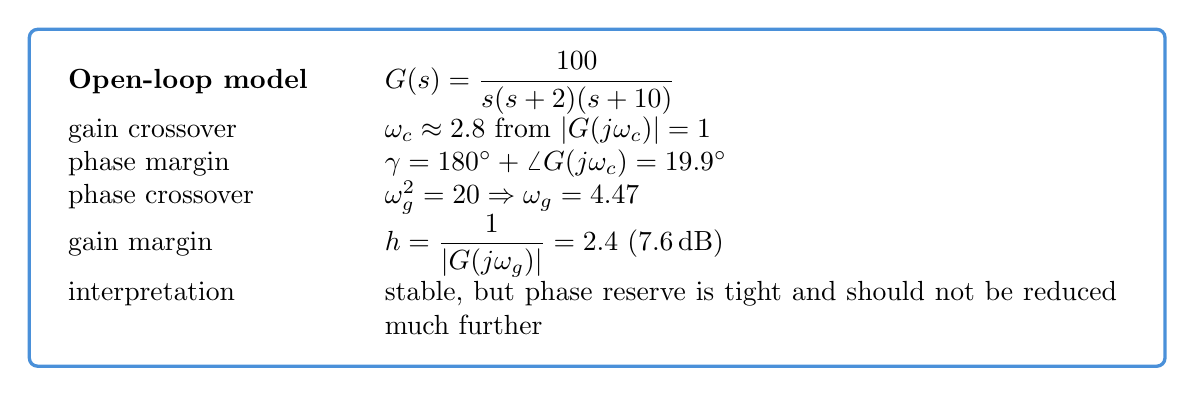
\begin{tikzpicture}[line width=1.2pt]
  \node[
    draw=blockblue,
    rounded corners=3pt,
    inner sep=8pt,
    align=left
  ] at (0,0) {
    \begin{tabular}{p{3.6cm}p{9.3cm}}
      \textbf{Open-loop model} & $\displaystyle G(s)=\frac{100}{s(s+2)(s+10)}$ \\
      gain crossover & $\omega_c \approx 2.8$ from $|G(j\omega_c)|=1$ \\
      phase margin & $\gamma = 180^\circ + \angle G(j\omega_c) = 19.9^\circ$ \\
      phase crossover & $\omega_g^2 = 20 \Rightarrow \omega_g = 4.47$ \\
      gain margin & $\displaystyle h=\frac{1}{|G(j\omega_g)|}=2.4\ (7.6\,\mathrm{dB})$ \\
      interpretation & stable, but phase reserve is tight and should not be reduced much further \\
    \end{tabular}
  };
\end{tikzpicture}
\end{document}
